\section{Implementation benchmarks}
The benchmarks presented in this section serve the purpose of assessing if the implementation is correct and is performing acceptably well.

\subsection{MHD Blast}
Similar benchmarks of spherical blast waves have been used in articles (\cite{blast1}, \cite{blast2}), and as a benchmark in software (\cite{athena} - \url{http://www.astro.princeton.edu/~jstone/Athena/tests/blast/blast.html} ).


\paragraph{Description}
Different authors set this problem up in different ways. We took the form that was used to test \cite{athena}, and extended it from 2 to 3 dimensions. The description is the following:
\begin{itemize}
    \item $\Omega = \lb-0.5, 0.5\rb \times \lb-0.75, 0.75\rb \times \{0\}$
    \item $\gamma = 1.4$
    \item Outflow condition everywhere on $\Gamma_B$
    \item Initial conditions:
    \begin{itemize}
        \item $\rho = 1.0$
        \item $p\lo\bfx\ro = 10.0,\,x<0.1;\ p = 0.1$ elsewhere
        \item $\bfpi = 0,\,x>0.1$
        \item $\bfB = \lo\frac{1}{\sqrt{2}}, \frac{1}{\sqrt{2}}, 0\ro$
    \end{itemize}
   \end{itemize}

\subsubsection{Calculation specification}
A mesh $T_h$ formed by 400 x 600 x 1 rectangular parallelepipeds was used.
The value of the time step $\tau$ used was set according to the CFL condition (\ref{section:CFL}) and was $\approx 10^{-7}$.
Illustration of the obtained results follows below - these results were obtained using one node of the department's computational cluster with these parameters:
\begin{itemize}
    \item CPU: 2 x Intel(R) Xeon(R) CPU E5-2680 v3 @ 2.50GHz
    \item \# of Cores: 48
    \item Vectorization support: AVX2
    \item Parallelization implemented: Intel TBB
    \item RAM: 512 GB
    \item OS: Ubuntu 15.10
\end{itemize}

\subsubsection{Results}
The results show distribution of plasma - $\rho$ in the domain.
\begin{figure}[H]
\begin{center}
    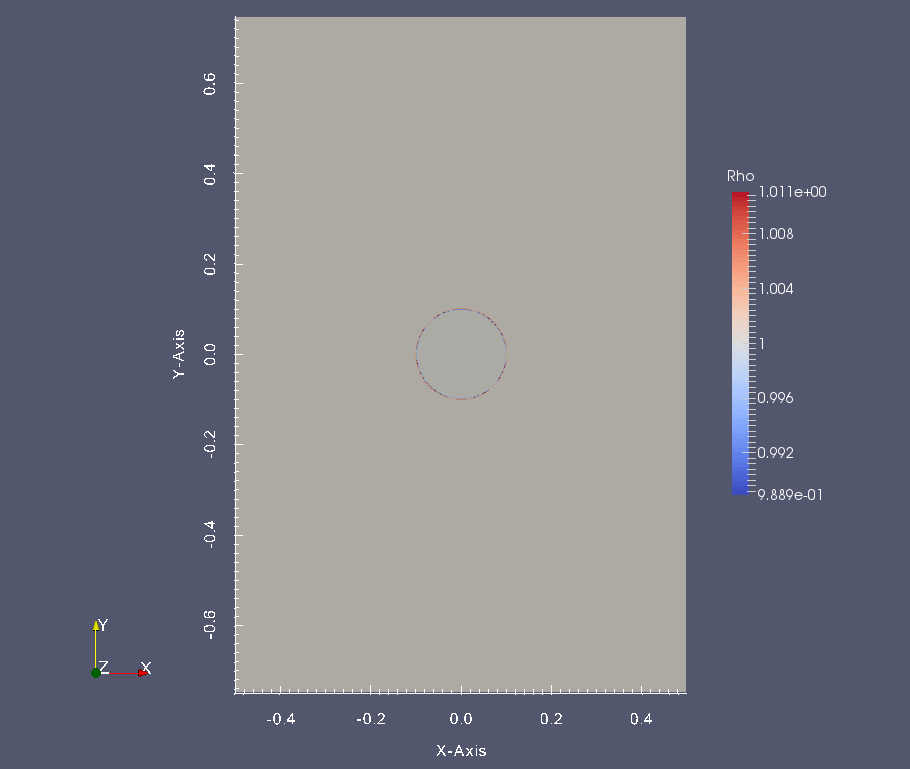
\includegraphics[width=0.4\textwidth]{img/0-density.png}
    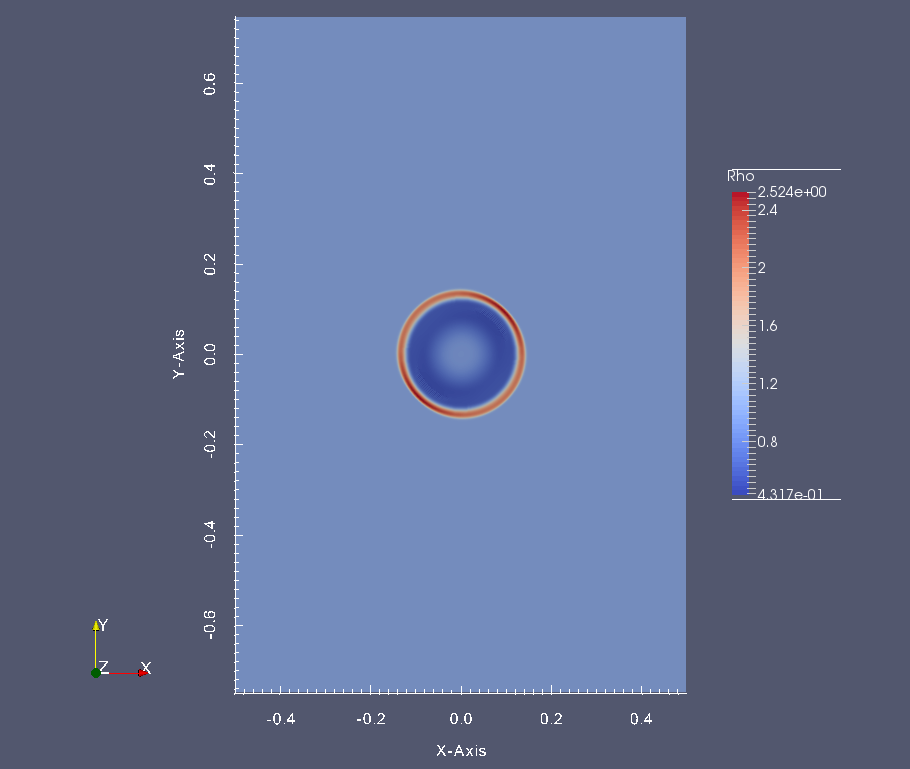
\includegraphics[width=0.4\textwidth]{img/5-density.png}
\end{center} 
\caption{Plasma density in $t = 0$ and $t = 0.03s$.}
\end{figure} 
\begin{figure}[H]
    \begin{center}
        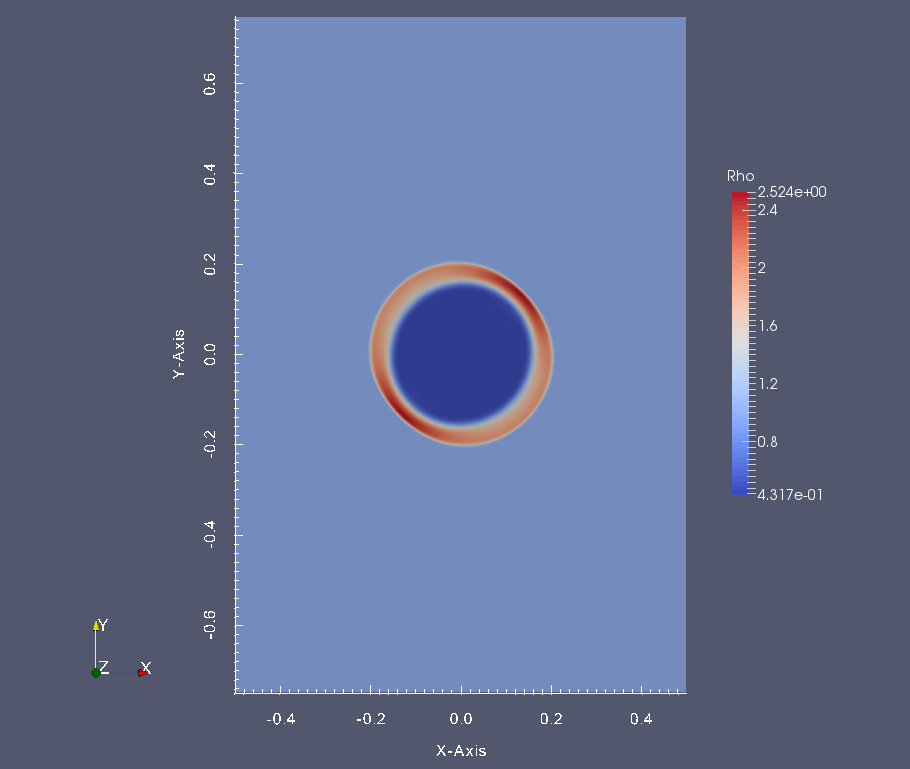
\includegraphics[width=0.4\textwidth]{img/10-density.png}
        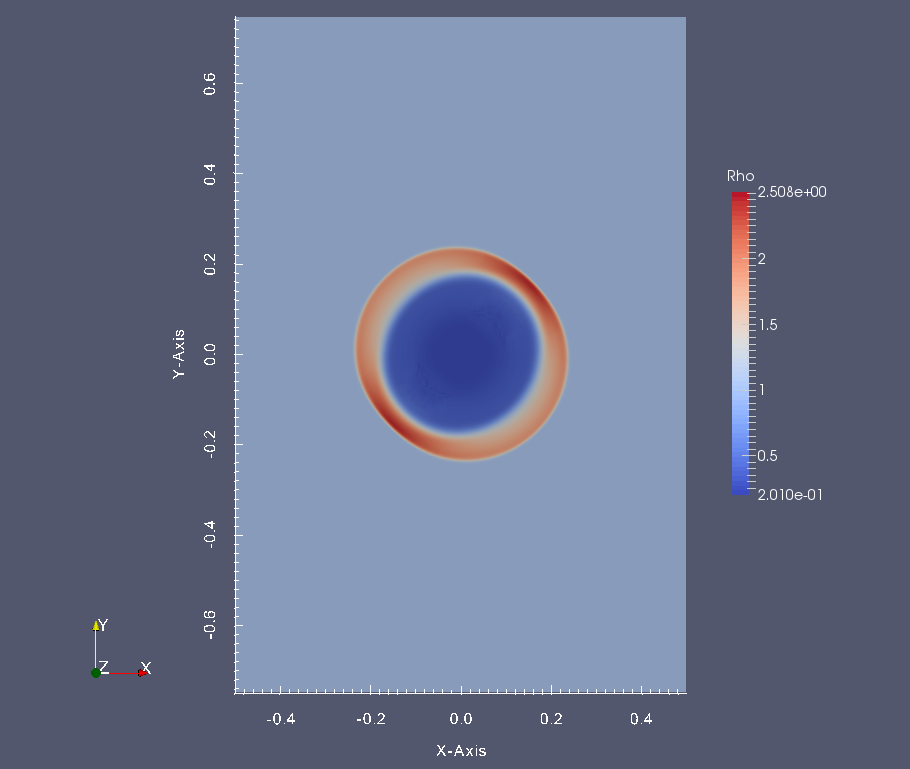
\includegraphics[width=0.4\textwidth]{img/13-density.png}
    \end{center} 
    \caption{Plasma density in $t = 0.12s$ and $t = 0.16s$.}
\end{figure} 
\begin{figure}[H]
    \begin{center}
        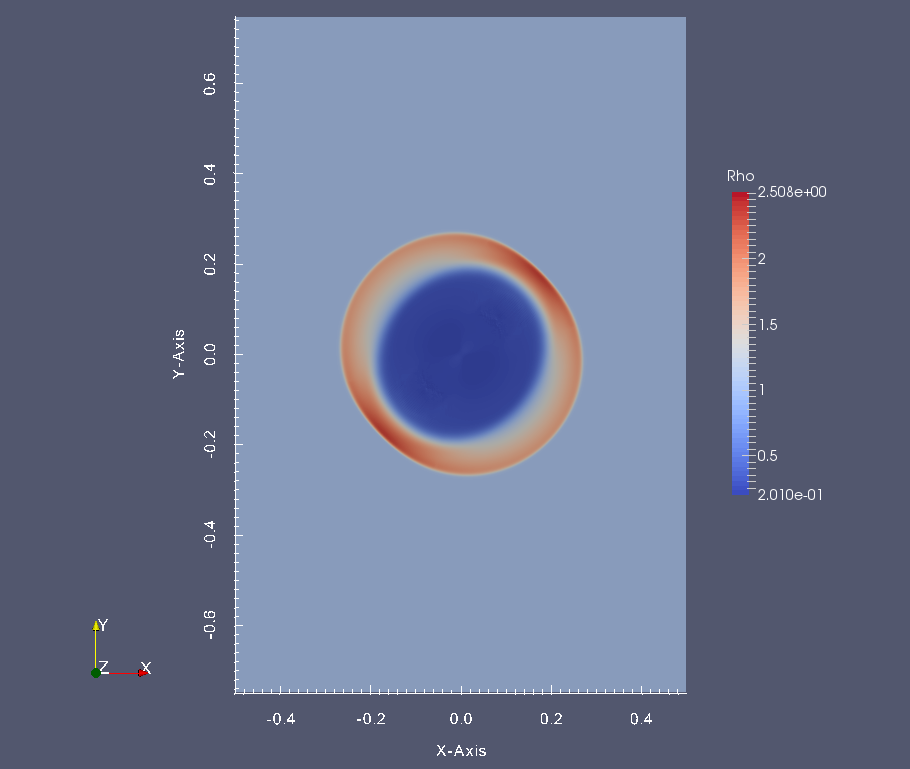
\includegraphics[width=0.4\textwidth]{img/16-density.png}
        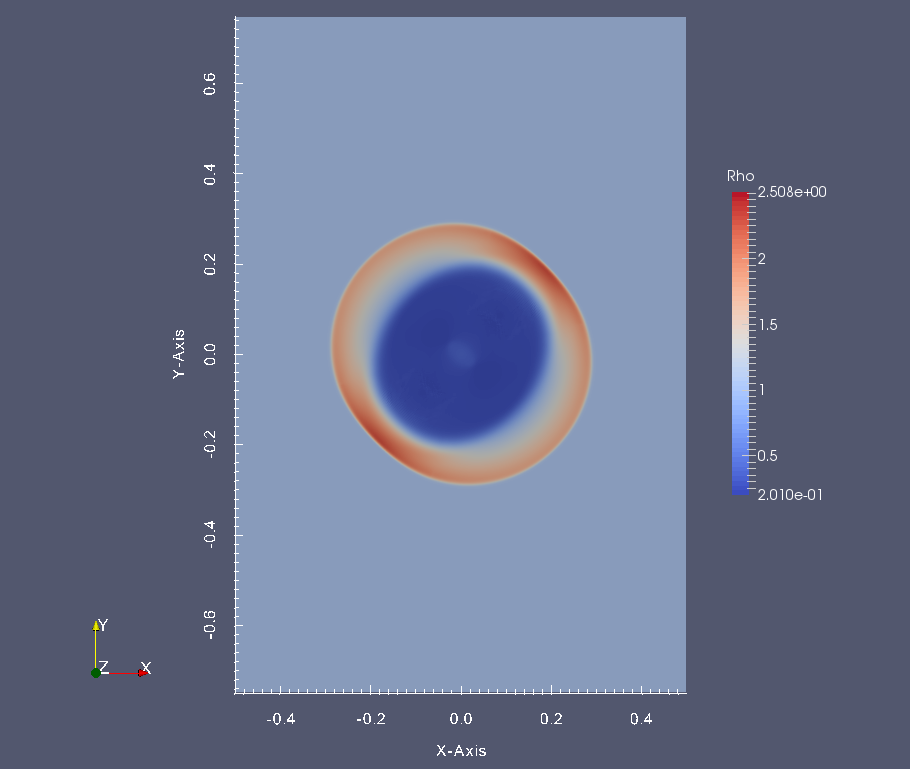
\includegraphics[width=0.4\textwidth]{img/18-density.png}
    \end{center} 
    \caption{Plasma density in $t = 0.19s$ and $t = 0.21s$.}
\end{figure} 
\begin{figure}[H]
    \begin{center}
        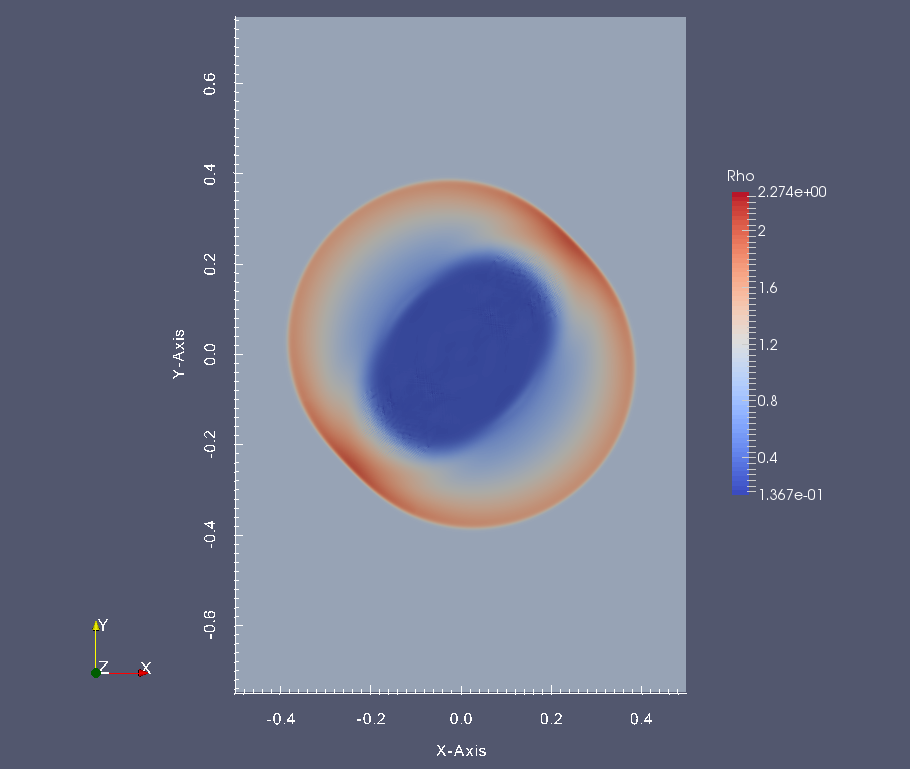
\includegraphics[width=0.4\textwidth]{img/20-density.png}
        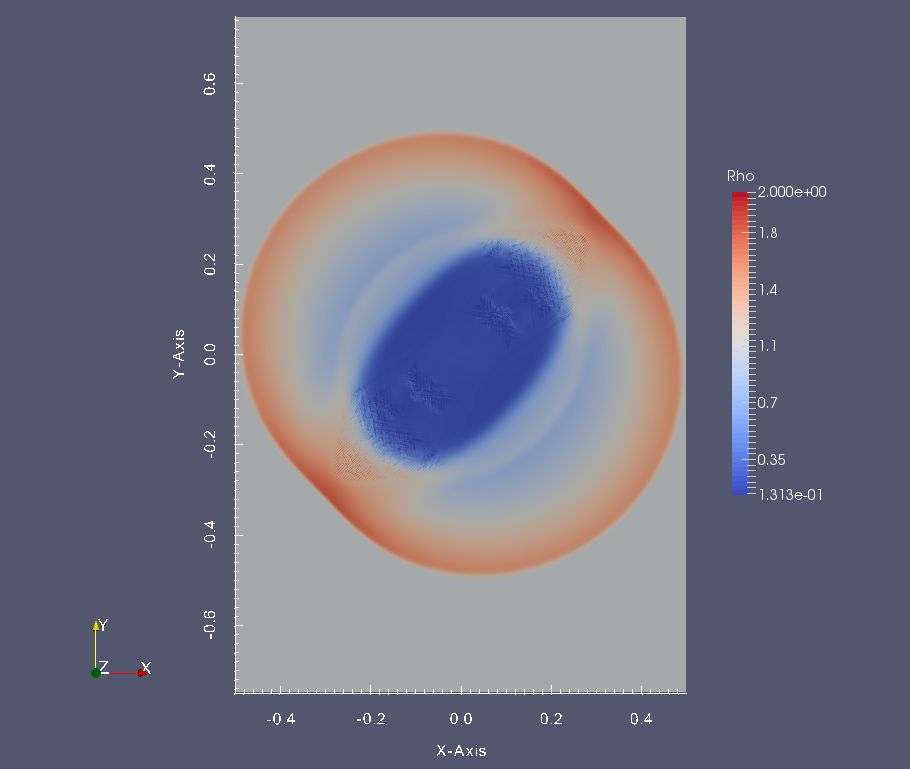
\includegraphics[width=0.4\textwidth]{img/21-density.png}
    \end{center} 
    \caption{Plasma density in $t = 0.32s$ and $t = 0.37s$.}
\end{figure} 

\subsection{Conclusions}
Results are satisfactory in terms of both qualitative and quantitative evaluation. Some non-physical instabilities are present - which will be subject to further study. Generally, results show good agreement with the expected results. The implementation has been proven to be working in an efficient manner, but challenges of real world large-scale problems lie ahead. There is still room for performance improvement, and for implementation of improved algorithms alike, especially with focus on stabilization of the implemented algorithm.